\documentclass[8pt,landscape]{article}
%\usepackage{pslatex}
\usepackage{graphicx}
\usepackage{multicol}
\usepackage{calc}
\usepackage{color}

\usepackage{hyperref}
\usepackage[]{url}
\hypersetup{%
  colorlinks=true,  
  linkcolor = black,
  citecolor = black, 
  urlcolor = blue, 
  pdfpagemode=UseNone, 
  pdfstartview=FitH,
  pdfauthor= {Jonas Stein, Tom Short, Emanuel Paradis},
  pdftitle= R Reference Card
}

\urlstyle{same}


% Turn off header and footer
\pagestyle{empty}

%\setlength{\leftmargin}{0.75in}
\setlength{\oddsidemargin}{-0.75in}
\setlength{\evensidemargin}{-0.75in}
\setlength{\textwidth}{10.5in}


\setlength{\topmargin}{-0.2in}
\setlength{\textheight}{7.4in}
\setlength{\headheight}{0in}
\setlength{\headsep}{0in}

\pdfpageheight\paperheight
\pdfpagewidth\paperwidth

% Redefine section commands to use less space
\makeatletter
\renewcommand\section{\@startsection{section}{1}{0mm}%
                                     {-24pt}% \@plus -12pt \@minus -6pt}%
                                     {0.5ex}%
                                {\color{blue}\normalfont\large\bfseries}}
\makeatother

% Don't print section numbers
\setcounter{secnumdepth}{0}

\setlength{\parindent}{0pt}
\setlength{\parskip}{0pt}

\newcommand{\code}{\texttt}
\newcommand{\bcode}[1]{\texttt{\textbf{#1}}}
\newcommand\F{\code{FALSE}}
\newcommand\T{\code{TRUE}}

%\newcommand{\hangpara}[2]{\hangindent#1\hangafter#2\noindent}
%\newenvironment{hangparas}[2]{\setlength{\parindent}{\z@}\everypar={\hangpara{#1}{#2}}}

\newcommand{\describe}[1]{\begin{description}{#1}\end{description}}


% -----------------------------------------------------------------------

\begin{document}

%\raggedright
\footnotesize
\begin{multicols*}{3}

% multicol parameters
% These lengths are set only within the two main columns
%\setlength{\columnseprule}{0.25pt}
\setlength{\premulticols}{1pt}
\setlength{\postmulticols}{1pt}
\setlength{\multicolsep}{1pt}
\setlength{\columnsep}{2pt}

\begin{center}
     {\Large{\textbf{\color{blue}R Reference Card}}} \\
 \today
\end{center}
\href{mailto:news@jonasstein.de}{Jonas Stein} maintains 
the source since 2012 on \href{https://github.com/jonasstein/R-Reference-Card}{github} feel free to contact him for contributions.
Parent versions by Tom Short, includes material from 
\href{http://cran.r-project.org/doc/contrib/Paradis-rdebuts_en.pdf}{R for Beginners} 
by courtesy of Emmanuel Paradis.\\

Examples in this document use the variables \code{df} = data frame object, \code{v} = vector, \code{s} = string,  \code{f} = filename as string all others are not yet rewritten.

\section{Getting help}
\everypar={\hangindent=9mm}

\bcode{help(topic)} documentation on \code{topic} 

\bcode{?topic} short alternative to \code{help}

\bcode{?.Machine} help about maximum values on your machine

\bcode{help.search("topic")} search the help system 

\bcode{apropos("topic")} the names of all objects in the search list
matching the regular expression "topic"

\bcode{help.start()} start the HTML version of help

\bcode{str(a)} display the internal structure of an R object

\bcode{summary(a)} gives a ``summary'' of \code{a}, usually a
statistical summary but it is \emph{generic} meaning it has different operations for different
classes of \code{a}

\bcode{ls()} show objects in the search path; specify \code{pat="pat"}
to search on a pattern

\bcode{ls.str()} str() for each variable in the search path

\bcode{dir()} show files in the current directory

\bcode{methods(a)} shows S3 methods of \code{a}

\bcode{methods(class=class(a))} lists all the methods to handle objects
of class a




\section{Input and output}
\everypar={\hangindent=9mm}

\bcode{source("my.R")} includes and executes my.R in this place

\bcode{data(f)} loads specified data sets

\bcode{library(s)} load add-on packages

\bcode{read.table(f)} reads a file in table format and
                creates a data frame from it; the default separator
                \code{sep=""} is any whitespace; use \code{header=TRUE}
                to read the first line as a header of column names; use \code{as.is=TRUE} to
                prevent character vectors from being converted to
                factors; use \code{comment.char=""} to prevent
                \code{"\#"} from being interpreted as a comment; use
                \code{skip=n} to skip \code{n} lines before reading data; see
                the help for options on row naming, NA treatment, and
                others

\bcode{read.csv(f,header=TRUE)} id. but with defaults set for reading
comma-delimited files

\bcode{read.delim(f",header=TRUE)} id. but with defaults set for reading
tab-delimited files

\bcode{read.fwf(f,widths,header=FALSE,sep="\t",as.is=FALSE)} read a table of \emph{f}ixed \emph{w}idth \emph{f}ormatted data into a
     'data.frame'; \code{widths} is an integer vector, giving the widths of the fixed-width fields


\bcode{save(f,...)} saves the specified objects (...) in the XDR
platform-independent binary format

\bcode{save.image(f)} saves all objects

\bcode{load(f)} load the datasets written with \code{save}


\bcode{cat(..., file=f, sep=" ")} prints the arguments after coercing to
character; \code{sep} is the character separator between arguments

\bcode{print(a, ...)} prints its arguments; generic, meaning it can
have different methods for different objects

\bcode{format(x,...)} format an R object for pretty printing

\bcode{write.table(x, file=f,row.names=TRUE, col.names=TRUE, sep=" ")} 
prints \code{x} after converting to a data frame; if \code{quote} is
                 \code{TRUE}, character or factor columns are
                 surrounded by quotes (\code{"}); \code{sep} is the field
                 separator; \code{eol} is the end-of-line separator;
                 \code{na} is the string for missing values; use
                 \code{col.names=NA} to add a blank column header to
                 get the column headers aligned correctly for
                 spreadsheet input

\bcode{sink(f)} output to \code{f}, until \code{sink()}

\everypar={\hangindent=0mm}
Most of the I/O functions have a \code{file} argument. This can often
be a character string naming a file or a connection.  \code{file=""} means the standard input or
output. Connections can include files, pipes, zipped
files, and R variables. 

On windows, the file connection can also be used with \code{description =
"clipboard"}. To exchange tables with office applications via clipboard, use \\
\code{x <- read.delim("clipboard")}\\
\code{write.table(x,"clipboard",sep="\textbackslash t",col.names=NA)}

For database interaction, see packages \code{RODBC}, \code{DBI},
\code{RMySQL}, \code{RPgSQL}, \code{ROracle}, for other file formats see
\code{XML}, \code{hdf5}, \code{netCDF} 




\section{Data creation}
\everypar={\hangindent=9mm}

\bcode{c(...)} generic function to combine arguments with the default
forming a vector;
with \code{recursive=TRUE} descends through lists combining all elements
into one vector

\bcode{from:to} generates a sequence; ``:'' has operator priority; 1:4
+ 1 is ``2,3,4,5''

\bcode{seq(from,to)} generates a sequence
\code{by=} specifies increment; \code{length=} specifies desired length

\bcode{seq(along=x)} generates \code{1, 2, ..., length(along)}; useful for
\code{for} loops

\bcode{rep(x,times)} replicate \code{x} \code{times}; use \code{each=}
to repeat ``each'' element of \code{x} \code{each} times;
\code{rep(c(1,2,3),2)} is 1 2 3 1 2 3; \code{rep(c(1,2,3),each=2)} is 1 1 2 2 3 3 

\bcode{data.frame(...)} create a data frame of the named or unnamed arguments;
  \code{data.frame(v=1:4,ch=c("a","B","c","d"),n=10)}; shorter vectors
  are recycled to the length of the longest 

\bcode{list(...)} create a list of the named or unnamed arguments;
  \code{list(a=c(1,2),b="hi",c=3i)}; 

\bcode{array(x,dim=)} array with data \code{x}; specify
dimensions like \code{dim=c(3,4,2)}; elements of \code{x} recycle if \code{x}
is not long enough

\bcode{matrix(x,nrow=,ncol=)} matrix; elements of \code{x} recycle

\bcode{factor(x,levels=)} encodes a vector \code{x} as a factor

\bcode{gl(n,k,length=n*k,labels=1:n)} generate levels (factors) by specifying
the pattern of their levels; \code{k} is the number of levels, and \code{n} is the
number of replications

\bcode{expand.grid()} a data frame from all combinations of the supplied vectors
     or factors

\bcode{rbind(...)} combine arguments by rows for matrices, data frames, and
others

\bcode{cbind(...)} id. by columns


\section{Data destruction}
\bcode{rm(myvar)} removes object \code{myvar} from memory

\bcode{rm(list = ls(all = TRUE))} removes all objects from memory

\section{addressing vectors}

\begin{tabular}{@{}l@{\ }l}
\code{v[n]} & \code{n}$^{th}$ element\\
\code{v[-n]} & all \emph{but} the \code{n}$^{th}$ element\\
\code{v[1:n]} & first \code{n} elements\\
\code{v[-(1:n)]} & elements from \code{n+1} to the end\\
\code{v[c(1,4,2)]} & specific elements\\
\code{v["name"]} & element named \code{"name"}\\
\code{v[x > 3]} & all elements greater than 3\\
\code{v[x > 3 \& x < 5]} & all elements between 3 and 5\\
\code{v[x \%in\% c("a","and","the")]} & elements in the given set\\
\end{tabular}

\section{addressing lists}
\samepage\begin{tabular}{@{}l@{\ }l}
\code{x[n]} & list with elements \code{n}\\
\code{x[[n]]} & \code{n}$^{th}$ element of the list\\
\code{x[["name"]]} & element of the list named \code{"name"}\\
\code{x\$name} & id.\\
\end{tabular}

\section{addressing matrices}
\begin{tabular}{@{}l@{\ }l}
\code{x[i,j]} & element at row \code{i}, column \code{j}\\
\code{x[i,]} & row \code{i}\\
\code{x[,j]} & column \code{j}\\
\code{x[,c(1,3)]} & columns 1 and 3\\
\code{x["name",]} & row named \code{"name"}\\
\end{tabular}

Indexing data frames (matrix indexing plus the following)

\begin{tabular}{@{}l@{\ }l}
\code{df[["name"]]} & column named \code{"name"}\\
\code{df\$name} & id.\\
\end{tabular}



\section{Variable conversion} 
\everypar={\hangindent=9mm}

\bcode{as.array(x), as.data.frame(x), as.numeric(x), as.logical(x),
as.complex(x), as.character(x), ...} convert type;  \code{methods(as)} 
shows a complete list
 


\section{Variable information} 
\everypar={\hangindent=9mm}

\bcode{is.na(x), is.null(x), is.array(x), is.data.frame(x), is.numeric(x),
  is.complex(x), is.character(x), ...} test for type; for a complete list,
  use \code{methods(is)}

\bcode{length(x)}  number of elements in \code{x}

\bcode{dim(x)} Retrieve or set the dimension of an object;
\code{dim(x) <- c(3,2)}

\bcode{dimnames(x)} Retrieve or set the dimension names of an object

\bcode{nrow(x)} number of rows; \code{NROW(x)} is the same but treats
a vector as a one-row matrix

\bcode{ncol(x)} and \bcode{NCOL(x)} id. for columns

\bcode{class(x)} get or set the class of \code{x}; \code{class(x) <- "myclass"}

\bcode{unclass(x)} remove the class attribute of \code{x}

\bcode{attr(x,which)} get or set the attribute \code{which} of \code{x}

\bcode{attributes(obj)} get or set the list of attributes of \code{obj}





\section{Data selection and manipulation}
\everypar={\hangindent=9mm}

\bcode{which.max(v), which.min(v)}  returns the index of the maximum (minimum) element of
\bcode{v}

\bcode{rev(v)}  reverses the elements of \code{v}

\bcode{sort(v)}  sorts the elements of \code{v} in increasing order; to sort in decreasing order: \code{rev(sort(x))}

\bcode{cut(x,breaks)}  divides \code{x} into intervals (factors);
\code{breaks} is the number of cut intervals or a vector of cut points

\bcode{match(x, y)}  returns a vector of the same length than \code{x} with the elements of \code{x} which are in \code{y} (\code{NA} otherwise)

\bcode{which(x == a)}  returns a vector of the indices of \code{x} if the comparison operation is true (\T), in this example the values of \code{i} for which \code{x[i] == a} (the argument of this function must be a variable of mode logical)

\bcode{choose(n, k)}  computes the combinations of $k$ events among $n$ repetitions = $n!/[(n-k)!k!]$

\bcode{na.omit(x)}  suppresses the observations with missing data (\code{NA}) (suppresses the corresponding line if \code{x} is a matrix or a data frame)

\bcode{na.fail(x)}  returns an error message if \code{x} contains at least one \code{NA}

\bcode{unique(x)}  if \code{x} is a vector or a data frame, returns a similar object but with the duplicate elements suppressed

\bcode{table(x)}  returns a table with the numbers of the differents values of \code{x} (typically for integers or factors)

\bcode{subset(x, ...)}  returns a selection of \code{x} with respect to criteria (\code{...}, typically comparisons: \code{x\$V1 < 10}); if \code{x} is a data frame, the option \code{select} gives the variables to be kept or dropped using a minus sign

\bcode{sample(x, size)}  resample randomly and without replacement \code{size} elements in the vector \code{x}, the option \code{replace = TRUE} allows to resample with replacement

\bcode{prop.table(x,margin=)} table entries as fraction of marginal table 




\section{Math}
\everypar={\hangindent=9mm}

\bcode{sin,cos,tan,asin,acos,atan,atan2,log,log10,exp}

\bcode{range(x)}  id. then \code{c(min(x), max(x))}

\bcode{sum(x)}  sum of the elements of \code{x}

\bcode{diff(x)}  lagged and iterated differences of vector \code{x}

\bcode{prod(x)}  product of the elements of \code{x}

\bcode{mean(x)}  mean of the elements of \code{x}

\bcode{median(x)}  median of the elements of \code{x}

\bcode{quantile(x,probs=)} sample quantiles
     corresponding to the given probabilities (defaults to 0,.25,.5,.75,1)

\bcode{weighted.mean(x, w)} mean of \code{x} with weights \code{w}

\bcode{rank(x)}  ranks of the elements of \code{x}

\bcode{var(x)} or \code{cov(x)}  variance of the elements of \code{x}
(calculated on $n-1$); if \code{x} is a matrix or a data frame, the
variance-covariance matrix is calculated

\bcode{sd(x)} standard deviation of \code{x}

\bcode{cor(x)}  correlation matrix of \code{x} if it is a matrix or a
data frame (1 if \code{x} is a vector)

\bcode{var(x, y)} or \code{cov(x, y)}  covariance between \code{x} and \code{y}, or between the columns of \code{x} and those of \code{y} if they are matrices or data frames

\bcode{cor(x, y)}  linear correlation between \code{x} and \code{y}, or correlation matrix if they are matrices or data frames

\bcode{round(x, n)}  rounds the elements of \code{x} to \code{n}
decimals

\bcode{log(v, base)}  computes the logarithm of \code{x} with base \code{base} 
\bcode{log10(v)}  \code{base} =10

\bcode{scale(x)}  if \code{x} is a matrix, centers and reduces the data; to center only use the option \code{center=FALSE}, to reduce only \code{scale=FALSE} (by default \code{center=TRUE, scale=TRUE})

\bcode{pmin(x,y,...)}  a vector which $i$th element is the minimum of \code{x[i]}, \code{y[i]}, \ldots

\bcode{pmax(x,y,...)}  id. for the maximum

\bcode{cumsum(v)}  a vector which $i$th element is the sum from \code{x[1]} to \code{x[i]}

\bcode{cumprod(v)}  $f_i = \Pi_{j=1..i} x_j = (x_1, x_1 \cdot x_2, \dots)$

\bcode{cummin(v)}  $f_i = \min(x_1 \dots x_i)$

\bcode{cummax(v)}  id. for the maximum

\bcode{union(x,y)},~\bcode{intersect(x,y)},~\bcode{setdiff(x,y)},~\bcode{setequal(x,y)}, \bcode{is.element(el,set)} ``set'' functions

\bcode{Re(z), Im(z)} real and imaginary part of a complex number

\bcode{Mod(z)} modulus; \code{abs(x)} is the same

\bcode{Arg(z)} angle in radians of the complex number

\bcode{Conj(z)} complex conjugate

\bcode{convolve(x,y)} compute the several kinds of
     convolutions of two sequences

\bcode{fft(v)} Fast Fourier Transform
\bcode{mvfft(x)} FFT of each column of a matrix

\bcode{filter(x,filter)} applies linear filtering to a univariate time series or to each
     series separately of a multivariate time series

\everypar={\hangindent=0mm}
Many math functions have a logical parameter \code{na.rm=FALSE} to
specify missing data (NA) removal.




\section{Matrices}
\everypar={\hangindent=9mm}

\bcode{t(x)} transpose

\bcode{diag(x)} diagonal

\bcode{\%*\%} matrix multiplication

\bcode{solve(a,b)} solves \code{a \%*\% x = b} for \code{x}

\bcode{solve(a)} matrix inverse of \code{a}

\bcode{rowsum(x)} sum of rows for a matrix-like object;
\bcode{rowSums(x)} is a faster version

\bcode{colsum(x)}, \bcode{colSums(x)} id. for columns

\bcode{rowMeans(x)} fast version of row means
\bcode{colMeans(x)} id. for columns


\section{Advanced data processing}
\everypar={\hangindent=9mm}

\bcode{apply(X,INDEX,FUN=)} a vector or array or list of values obtained by applying a
     function \code{FUN} to margins (\code{INDEX}) of \code{X}

\bcode{lapply(X,FUN)} apply \code{FUN} to each element of the list \code{X}

\bcode{tapply(X,INDEX,FUN=)} apply \code{FUN} to each cell
of a ragged array given by \code{X} with indexes \code{INDEX}

\bcode{by(data,INDEX,FUN)} apply \code{FUN} to data frame \code{data}
subsetted by \code{INDEX}

\bcode{merge(a,b)} merge two data frames by common columns or row names

\bcode{xtabs(a~b,data=x)} a contingency table from cross-classifying factors

\bcode{aggregate(x,by,FUN)} splits the data frame \code{x} into subsets, computes summary statistics for
     each, and returns the result in a convenient form; \code{by} is a
     list of grouping elements, each as long as the variables in \code{x}

\bcode{stack(x, ...)} transform data available as
     separate columns in a data frame or list into a single column

\bcode{unstack(x, ...)} inverse of \code{stack()}

\bcode{reshape(x, ...)} reshapes a data frame between 'wide' format with
     repeated measurements in separate columns of the same record and
     'long' format with the repeated measurements in separate records;
     use \code(direction="wide") or \code(direction="long")





\section{Strings}
\everypar={\hangindent=9mm}

\bcode{paste(s1,s2, sep=\" \")} concatenate vectors after converting to character; 
\code{collapse=} is an optional string to separate ``collapsed'' results
\bcode{paste0(s1,s2)} paste without seperator (since R 2.15)

\bcode{substr(s,start,stop)} substrings in a character vector; can also assign, as \code{substr(s, start, stop) <- value}

\bcode{strsplit(s,split)} split \code{s} according to the substring \code{split}

\bcode{grep(pattern,x)} searches for matches to \code{pattern}
     within \code{x}; see \code{?regex}

\bcode{gsub(pattern,replacement,x)} replacement of matches determined by
regular expression matching \code{sub()} is the same but only
replaces the first occurrence. 

\bcode{tolower(s), toupper(s)} convert to lowercase (uppercase)

\bcode{match(x,table)} a vector of the positions of first matches for the elements of \code{x} among \code{table}

\bcode{x \%in\% table} id. but returns a logical vector 

\bcode{pmatch(x,table)} partial matches for the elements of \code{x} among \code{table}

\bcode{nchar(s)} number of characters


\section{\color{blue}Dates and Times}

The class \code{Date} has dates without times.  \code{POSIXct} has
dates and times, including time zones. Comparisons (e.g. $>$),
\code{seq()}, and \code{difftime()} are useful. \code{Date} also allows
$+$ and $-$. \code{?DateTimeClasses} gives more information. See also package
\code{chron}.

\everypar={\hangindent=9mm}

\bcode{as.Date(s)} and \bcode{as.POSIXct(s)} convert to the respective
class; \code{format(dt)} converts to a string representation. The
default string format is ``2012-02-21''. These accept a second argument
to specify a format for conversion. Some common formats are:

  \describe{
\itemsep=0pt\parskip=0pt
    \item{\code{\%a}, \code{\%A}} {Abbreviated and full weekday name.}
    \item{\code{\%b}, \code{\%B}} {Abbreviated and full month name.}
    \item{\code{\%d}} {Day of the month (01--31).}
    \item{\code{\%H}} {Hours (00--23).}
    \item{\code{\%I}} {Hours (01--12).}
    \item{\code{\%j}} {Day of year (001--366).}
    \item{\code{\%m}} {Month (01--12).}
    \item{\code{\%M}} {Minute (00--59).}
    \item{\code{\%p}} {AM/PM indicator. }
    \item{\code{\%S}} {Second as decimal number (00--61).}
    \item{\code{\%U}} {Week (00--53); the first Sunday as day 1 of week 1.}
    \item{\code{\%w}} {Weekday (0--6, Sunday is 0).}
    \item{\code{\%W}} {Week (00--53); the first Monday as day 1 of week 1.}
    \item{\code{\%y}} {Year without century (00--99). Avoid it.}
    \item{\code{\%Y}} {Year with century.}
    \item{\code{\%z}} {(read only) Offset from Greenwich; \code{-0800} 
        is 8 hours west of.}
    \item{\code{\%Z}} {(read only) Time zone as a character string 
        (empty if not available).}
  }

Where leading zeros are shown they will be used on output but are
optional on input. See \code{?strftime}.  





\section{Plotting}

\everypar={\hangindent=9mm}

\bcode{plot(y)}  plot of the values of \code{y} (on the $y$-axis) ordered on the $x$-axis

\bcode{plot(x=xv, y=yv)}  bivariate plot of \code{xv} (on the $x$-axis) and \code{yv} (on the $y$-axis)

\bcode{hist(x)}  histogram of the frequencies of \code{x}

\bcode{barplot(x)}  histogram of the values of \code{x}; use
\code{horiz=FALSE} for horizontal bars

\bcode{dotchart(x)}  if \code{x} is a data frame, plots a Cleveland dot plot (stacked plots line-by-line and column-by-column)

\bcode{pie(x)}  circular pie-chart

\bcode{boxplot(x)}  ``box-and-whiskers'' plot

\bcode{sunflowerplot(x, y)}  id. than \code{plot()} but the points with similar coordinates are drawn as flowers which petal number represents the number of points

\bcode{stripplot(x)}  plot of the values of \code{x} on a line (an alternative to \code{boxplot()} for small sample sizes)

\bcode{coplot(x\~{}y $\mid$ z)}  bivariate plot of \code{x} and \code{y} for each value or interval of values of \code{z}

\bcode{interaction.plot (f1, f2, y)}  if \code{f1} and \code{f2} are factors, plots the means of \code{y} (on the $y$-axis) with respect to the values of \code{f1} (on the $x$-axis) and of \code{f2} (different curves); the option \code{fun} allows to choose the summary statistic of \code{y} (by default \code{fun=mean})

\bcode{matplot(x,y)}  bivariate plot of the first column of \code{x} {\it vs.} the first one of \code{y}, the second one of \code{x} {\it vs.} the second one of \code{y}, etc.

\bcode{fourfoldplot(x)}  visualizes, with quarters of circles, the association between two dichotomous variables for different populations (\code{x} must be an array with \code{dim=c(2, 2, k)}, or a matrix with \code{dim=c(2, 2)} if $k=1$)

\bcode{assocplot(x)}  Cohen--Friendly graph showing the deviations  from independence of rows and columns in a two dimensional contingency table

\bcode{mosaicplot(x)}  `mosaic' graph of the residuals from a log-linear regression of a contingency table

\bcode{pairs(x)}  if \code{x} is a matrix or a data frame, draws all possible bivariate plots between the columns of \code{x}

\bcode{plot.ts(x)}  if \code{x} is an object of class \code{"ts"}, plot of \code{x} with respect to time, \code{x}  may be multivariate but the series must have the same frequency and dates

\bcode{ts.plot(x)}  id. but if \code{x} is multivariate the series may have different dates and must have the same frequency

\bcode{qqnorm(x)}  quantiles of \code{x} with respect to the values expected under a normal law

\bcode{qqplot(x, y)}  quantiles of \code{y} with respect to the quantiles of \code{x}

\bcode{contour(x, y, z)}  contour plot (data are interpolated to draw the curves), \code{x} and \code{y} must be vectors and \code{z} must be a matrix so that \code{dim(z)=c(length(x), length(y))} (\code{x} and \code{y} may be omitted)

\bcode{filled.contour(x, y, z)}  id. but the areas between the contours are coloured, and a legend of the colours is drawn as well

\bcode{image(x, y, z)}  id. but with colours (actual data are plotted)

\bcode{persp(x, y, z)}  id. but in perspective (actual data are plotted)

\bcode{stars(x)}  if \code{x} is a matrix or a data frame, draws a graph with segments or a star where each row of \code{x} is represented by a star and the columns are the lengths of the segments

\bcode{symbols(x, y, ...)}  draws, at the coordinates given by \code{x} and \code{y}, symbols (circles, squares, rectangles, stars, thermometres or ``boxplots'') which sizes, colours \ldots{} are specified by supplementary arguments

\bcode{termplot(mod.obj)}  plot of the (partial) effects of a regression model (\code{mod.obj})

The following parameters are common to many plotting functions:

\bcode{add=FALSE}  if \T{} superposes the plot on the previous one (if it exists)

\bcode{axes=TRUE}  if \F{} does not draw the axes and the box

\bcode{type="p"}  specifies the type of plot, \code{"p"}: points, \code{"l"}: lines, \code{"b"}: points connected by lines, \code{"o"}: id. but the lines are over the points, \code{"h"}: vertical lines, \code{"s"}: steps, the data are represented by the top of the vertical lines, \code{"S"}: id. but the data are represented by the bottom of the vertical lines

\bcode{xlim=, ylim=}  specifies the lower and upper limits of the axes, for example with \code{xlim=c(1, 10)} or \code{xlim=range(x)}

\bcode{xlab=, ylab=}  annotates the axes, must be variables of mode character

\bcode{main=}  main title, must be a variable of mode character

\bcode{sub=}  sub-title (written in a smaller font)




\section{Low-level plotting commands}
\everypar={\hangindent=9mm}

\bcode{points(x, y)}  adds points (the option \code{type=} can be used)

\bcode{lines(x, y)}  id. but with lines

\bcode{text(x, y, \mbox{labels}, ...)}  adds text given by \code{labels} at coordinates (\code{x},\code{y}); a typical use is: \code{plot(x, y, type="n"); text(x, y, names)}

\bcode{mtext(text, side=3, line=0, ...)}  adds text given by \code{text} in the margin specified by \code{side} (see \code{axis()} below); \code{line} specifies the line from the plotting area

\bcode{segments(x0, y0, x1, y1)}  draws lines from points (\code{x0},\code{y0}) to points (\code{x1},\code{y1})

\bcode{arrows(x0, y0, x1, y1, angle= 30, code=2)}  id. with arrows at points (\code{x0},\code{y0}) if \code{code=2}, at points (\code{x1},\code{y1}) if \code{code=1}, or both if \code{code=3}; \code{angle} controls the angle from the shaft of the arrow to the edge of the arrow head

\bcode{abline(a,b)}  draws a line of slope \code{b} and intercept \code{a}

\bcode{abline(h=y)}  draws a horizontal line at ordinate \code{y}

\bcode{abline(v=x)}  draws a vertical line at abcissa \code{x}

\bcode{abline(lm.obj)}  draws the regression line given by \code{lm.obj}

\bcode{rect(x1, y1, x2, y2)}  draws a rectangle which left, right, bottom, and top limits are \code{x1}, \code{x2}, \code{y1}, and \code{y2}, respectively

\bcode{polygon(x, y)}  draws a polygon linking the points with coordinates given by \code{x} and \code{y}

\bcode{legend(x, y, legend)}  adds the legend at the point (\code{x},\code{y}) with the symbols given by \code{legend}

\bcode{title()}  adds a title and optionally a sub-title

\bcode{axis(side, vect)}  adds an axis at the bottom (\code{side=1}), on the left (\code{2}), at the top (\code{3}), or on the right (\code{4}); \code{vect} (optional) gives the abcissa (or ordinates) where tick-marks are drawn

\bcode{rug(x)}  draws the data \code{x} on the $x$-axis as small vertical lines

\bcode{locator(n, type="n", ...)}  returns the coordinates ($x,y$) after the user has clicked \code{n} times on the plot with the mouse; also draws symbols (\code{type="p"}) or lines (\code{type="l"}) with respect to optional graphic parameters (\code{...}); by default nothing is drawn (\code{type="n"})




\section{Graphical parameters}

These can be set globally with \bcode{par(...)}; many can be passed as
parameters to plotting commands.

\everypar={\hangindent=9mm}

\bcode{adj}  controls text justification (\code{0} left-justified, \code{0.5} centred, \code{1} right-justified)

\bcode{bg}  specifies the colour of the background (ex. : \code{bg="red"}, \code{bg="blue"}, \ldots{} the list of the 657 available colours is displayed with \code{colors()})

\bcode{bty}  controls the type of box drawn around the plot, allowed values are: \code{"o"}, \code{"l"}, \code{"7"}, \code{"c"}, \code{"u"} ou \code{"]"} (the box looks like the corresponding character); if \code{bty="n"} the box is not drawn

\bcode{cex}  a factor controlling the default size of texts and symbols; you can scale numbers on the axes, \code{cex.axis}, the axis labels, \code{cex.lab}, the title, \code{cex.main}, and the sub-title, \code{cex.sub}

\bcode{col}  controls the color of symbols and lines; use color names:
\code{"red"}, \code{"blue"} see \code{colors()} or as \code{"\#RRGGBB"};
see \code{rgb()}, \code{hsv()}, \code{gray()}, and \code{rainbow()}; as for \code{cex} there are: \code{col.axis}, \code{col.lab}, \code{col.main}, \code{col.sub}

\bcode{font}  an integer which controls the style of text (\code{1}: normal, \code{2}: italics, \code{3}: bold, \code{4}: bold italics); as for \code{cex} there are: \code{font.axis}, \code{font.lab}, \code{font.main}, \code{font.sub}

\bcode{las}  an integer which controls the orientation of the axis labels (\code{0}: parallel to the axes, \code{1}: horizontal, \code{2}: perpendicular to the axes, \code{3}: vertical)

\bcode{lty}  controls the type of lines, can be an integer or string (\code{1}: \code{"solid"}, \code{2}: \code{"dashed"}, \code{3}: \code{"dotted"}, \code{4}: \code{"dotdash"}, \code{5}: \code{"longdash"}, \code{6}: \code{"twodash"}, or a string of up to eight characters (between \code{"0"} and \code{"9"}) which specifies alternatively the length, in points or pixels, of the drawn elements and the blanks, for example \code{lty="44"} will have the same effect than \code{lty=2}

\bcode{lwd}  a numeric which controls the width of lines, default \code{1}

\bcode{mar}  a vector of 4 numeric values which control the space between the axes and the border of the graph of the form \code{c(bottom, left, top, right)}, the default values are \code{c(5.1, 4.1, 4.1, 2.1)}

\bcode{mfcol}  a vector of the form \code{c(nr,nc)} which partitions the graphic window as a matrix of \code{nr} lines and \code{nc} columns, the plots are then drawn in columns

\bcode{mfrow}  id. but the plots are drawn by row

\bcode{pch}  controls the type of symbol, either an integer between 1
and 25, or any single character within \code{""}

\samepage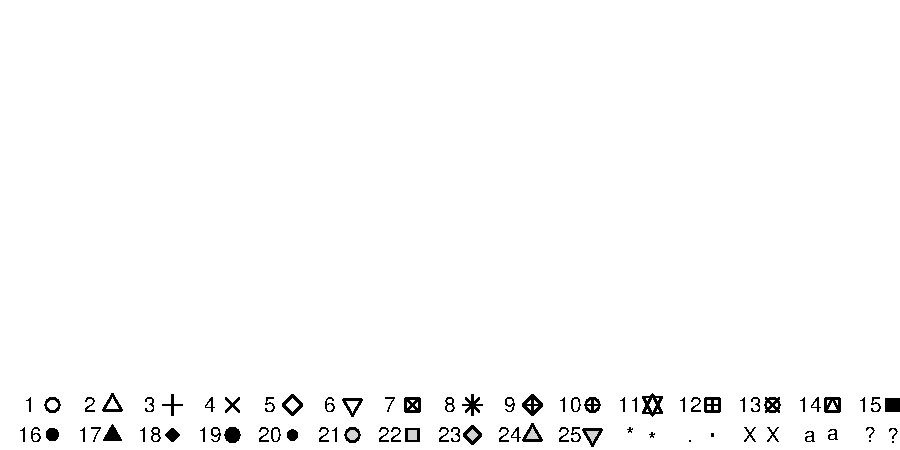
\includegraphics[width=8.5cm]{pch_symbol} 

\bcode{ps}   size in points of texts and symbols as integer

\bcode{pty}  a character which specifies the type of the plotting region, \code{"s"}: square, \code{"m"}: maximal

\bcode{tck}  a value which specifies the length of tick-marks on the axes as a fraction of the smallest of the width or height of the plot; if \code{tck=1} a grid is drawn

\bcode{tcl}  a value which specifies the length of tick-marks on the axes as a fraction of the height of a line of text (by default \code{tcl=-0.5})

\bcode{xaxt}  if \code{xaxt="n"} the $x$-axis is set but not drawn (useful in conjonction with \code{axis(side=1, ...)})

\bcode{yaxt}  if \code{yaxt="n"} the $y$-axis is set but not drawn (useful in conjonction with \code{axis(side=2, ...)})





\section{Lattice (Trellis) graphics}
\everypar={\hangindent=9mm}

\bcode{xyplot(y\~{}x)}  bivariate plots (with many functionalities)

\bcode{barchart(y\~{}x)}  histogram of the values of \code{y} with
respect to those of \code{x}

\bcode{dotplot(y\~{}x)}  Cleveland dot plot (stacked plots line-by-line
and column-by-column)

\bcode{densityplot(\~{}x)}  density functions plot

\bcode{histogram(\~{}x)}  histogram of the frequencies of \code{x}

\bcode{bwplot(y\~{}x)}  ``box-and-whiskers'' plot

\bcode{qqmath(\~{}x)}  quantiles of \code{x} with respect to the values expected under a theoretical distribution

\bcode{stripplot(y\~{}x)}  single dimension plot, \code{x} must be numeric, \code{y} may be a factor

\bcode{qq(y\~{}x)}  quantiles to compare two distributions, \code{x} must be numeric, \code{y} may be numeric, character, or factor but must have two `levels'

\bcode{splom(\~{}x)}  matrix of bivariate plots

\bcode{parallel(\~{}x)}  parallel coordinates plot

\bcode{levelplot(z\~{}x*y|g1*g2)}  coloured plot of the values of \code{z} at the coordinates given by \code{x} and \code{y} (\code{x}, \code{y} and \code{z} are all of the same length)

\bcode{wireframe(z\~{}x*y|g1*g2)}  3d surface plot

\bcode{cloud(z\~{}x*y|g1*g2)}  3d scatter plot

\everypar={\hangindent=0mm}
In the normal Lattice formula, \code{y~x|g1*g2} has
combinations of optional conditioning variables \code{g1}
and \code{g2} plotted on separate panels. Lattice functions 
take many of the same arguments as base
graphics plus also \code{data=} the data frame for the formula
variables and \code{subset=} for subsetting. Use \code{panel=} to
define a custom panel function (see \code{apropos("panel")}
and \code{?llines}). Lattice functions return an object of class
trellis and have to be \code{print}-ed to produce the graph. Use
\code{print(xyplot(...))} inside functions where automatic
printing doesn't work. Use \code{lattice.theme} and \code{lset} to
change Lattice defaults.



\section{Optimization and model fitting}
\everypar={\hangindent=9mm}

\bcode{optim(par, fn, method = c("Nelder-Mead", "BFGS", "CG",
  "L-BFGS-B", "SANN")} general-purpose optimization; \code{par} is
  initial values, \code{fn} is function to optimize (normally minimize)

\bcode{nlm(f,p)} minimize function \code{f} using a Newton-type
algorithm with starting values \code{p}

\bcode{lm(formula)} fit linear models; \code{formula} is typically of
     the form \code{response ~ termA + termB + ...}; use \code{I(x*y)
     + I(x\^{}2)} for terms made of nonlinear components

\bcode{glm(formula,family=)} fit generalized linear models, specified by
     giving a symbolic description of the linear predictor and a
     description of the error distribution; \code{family} is a
     description of the error distribution and link function to
          be used in the model; see \code{?family}

\bcode{nls(formula)} nonlinear least-squares estimates of the nonlinear
     model parameters

\bcode{approx(x,y=)} linearly interpolate given data points; \code{x} can be an
xy plotting structure

\bcode{spline(x,y=)} cubic spline interpolation

\bcode{loess(formula)} fit a polynomial surface using local fitting

\everypar={\hangindent=0mm}
Many of the formula-based modeling functions have several common
arguments: \code{data=} the data frame for the formula variables,
\code{subset=} a subset of variables used in the fit,
\code{na.action=} action for missing values: \code{"na.fail"}, \code{"na.omit"}, or
a function. The following generics often apply to model fitting functions: 

\everypar={\hangindent=9mm}
\bcode{predict(fit,...)}  predictions from \code{fit} based on input data

\bcode{df.residual(fit)}  returns the number of residual degrees of freedom

\bcode{coef(fit)}  returns the estimated coefficients (sometimes with their standard-errors)

\bcode{residuals(fit)}  returns the residuals

\bcode{deviance(fit)}  returns the deviance

\bcode{fitted(fit)}  returns the fitted values

\bcode{logLik(fit)}  computes the logarithm of the likelihood and the number of parameters

\bcode{AIC(fit)}  computes the Akaike information criterion or AIC


\section{Statistics}
\everypar={\hangindent=9mm}

\bcode{aov(formula)} analysis of variance model

\bcode{anova(fit,...)} analysis of variance (or deviance) tables for one or more
     fitted model objects

\bcode{density(x)} kernel density estimates of \code{x}

\bcode{binom.test()}, \bcode{pairwise.t.test()}, \bcode{power.t.test()},
\bcode{prop.test()}, \bcode{t.test()}, ... use
\code{help.search("test")} 





\section{Distributions}

\bcode{rnorm(n, mean=0, sd=1)} Gaussian (normal)  

\bcode{rexp(n, rate=1)} exponential

\bcode{rgamma(n, shape, scale=1)} gamma  

\bcode{rpois(n, lambda)} Poisson

\bcode{rweibull(n, shape, scale=1)} Weibull

\bcode{rcauchy(n, location=0, scale=1)} Cauchy  

\bcode{rbeta(n, shape1, shape2)} beta

\bcode{rt(n, df)} `Student' ($t$)  

\bcode{rf(n, df1, df2)} Fisher--Snedecor ($F$)  ($\chi^2$)  

\bcode{rchisq(n, df)} Pearson 

\bcode{rbinom(n, size, prob)} binomial  

\bcode{rgeom(n, prob)} geometric  

\bcode{rhyper(nn, m, n, k)} hypergeometric  

\bcode{rlogis(n, location=0, scale=1)} logistic  

\bcode{rlnorm(n, meanlog=0, sdlog=1)} lognormal  

\bcode{rnbinom(n, size, prob)} negative binomial  

\bcode{runif(n, min=0, max=1)} uniform  

\bcode{rwilcox(nn, m, n)}, \code{rsignrank(nn, n)} Wilcoxon's statistics  

All these functions can be used by replacing the letter \code{r} with
\code{d}, \code{p} or \code{q} to get, respectively, the probability
density (\code{d\textsl{func}(x, ...)}), the cumulative probability
density (\code{p\textsl{func}(x, ...)}), and the value of quantile
(\code{q\textsl{func}(p, ...)}, with 0 $<$ \code{p} $<$ 1).





\section{Programming}
\everypar={\hangindent=9mm}

\bcode{function( arglist ) expr} function definition

\bcode{return(value)}

\everypar={\hangindent=0mm}
\bcode{if(cond) expr\\
if(cond) cons.expr  else  alt.expr\\
for(var in seq) expr\\
while(cond) expr\\
repeat expr\\
break\\
next}

Use braces \{\} around statements


\everypar={\hangindent=9mm}
\bcode{ifelse(test, yes, no)} a value with the same shape as \code{test} filled with elements
from either \code{yes} or \code{no} 

\bcode{do.call(funname, args)} executes a function call from the name of
  the function and a list of arguments to be passed to it

\end{multicols*}
\end{document}
